% !TEX root = manuscript.tex
\documentclass{acm_proc_article-sp}
  %\documentclass{sig-alternate}
  
  \usepackage{latexsym}
  \usepackage{graphicx}
  \usepackage{amsmath}
  \usepackage{url}
  \usepackage[numbers]{natbib}
  \renewcommand{\vec}[1]{\mathbf{#1}}
  
  
  \makeatletter
  \let\@copyrightspace\relax
  \makeatother
  \title{DETECTING ALTERATION OF TIME-SERIES DATA USING PREDICTIVE CONVOLUTIONAL NEURAL NETWORKS}
  
  \numberofauthors{2}
  
  \author{
  \alignauthor
  Samuel B. Johnson\\
    \affaddr{Dept.\ of Computer Sci.\ \& Eng.}\\
    \affaddr{University of North Texas}
  % 2nd. author
  \alignauthor
  Ian Parberry\\
    \affaddr{Dept.\ of Computer Sci.\ \& Eng.}\\
    \affaddr{University of North Texas}
  }
  % \date{}
  
  \begin {document} \sloppy
  \maketitle
  
  \begin{abstract} 
  ABSTRACT GOES HERE.
  \end{abstract}
  
  \category{I.2.6}{Learning}{Machine Learning}
  
  \terms{Algorithms, Neural Networks, Signals}
  
  \keywords{Algorithms, Neural Networks, Signals}
  
  \section{Introduction}  
  \label{sec:intro}
  
  We consider the problem of detecting corruption, alteration, or insertion of data in time-series signals with multiple learnable features using neural networks. Convolutional neural networks (CNNs) are good at learning features of signals and predicting their sequences. We propose two methods of using CNNs to detect this. The first approach is intuitive and works with sufficient data, while the second is a novel method which demonstrates effectiveness with significantly less data. We also examine how these methods change along different hyperparameter axes.
  
  \section{Related Work / Background} 
  \label{sec:relatedWork}
  
  The original inspiration of this project, and a real-world example problem is the recent system called Rook~\cite{vines2015rook}, which inserts hidden messages into the network traffic of online multiplayer computer games, with the goal of censorship-resistant covert communication. The system analyzes the game traffic over time to identify byte positions in network packets that can be altered such that the recipient still considers it a valid game packet. These are called "mutable values," and are altered in such a way and frequency that the statistical properties are negligibly changed. Thus Rook is resistant to traditional detection approaches like statistical analysis.
  
  If we consider the game traffic to be a composition of signals with learnable patterns, then the mutable value alterations are interruptions in these patterns. Convolutional neural networks are effective at learning and predicting signals like this. In particular, Wavenet~\cite{DBLP:journals/corr/OordDZSVGKSK16} demonstrated the effectiveness of stacked dilated convolutional layers for generating audio, which is just a sum of periodic signals with learnable patterns.
  
  \section{Network}
  \label{sec:network}
  
  The network (Figure \ref{fig.model}) we use maps an input tensor of shape \((seqLength \times numFeatures)\) to an output of shape \((seqLength \times numFeatures)\) using 4 causal dilated convolutional layers with filter size \(numFeatures\); kernel size 4; and dilation rates 1, 2, 4, and 8, respectively. There is a final time distributed dense layer. The model uses tanh activation for all layers, mean squared error loss function, and adam optimizer. The input tensor is a sequence taken from our data. Where the feature vector at position \(i\) of the input tensor corresponds to position \(j\) of the overall signal, the \(i^{th}\) vector of the output tensor corresponds to position \(j+1\). The training and target data is split into blocks of size \((seqLength \times numFeatures)\). This network design could train all of the blocks in parallel per epoch, but we train with a batch size of 1, updating the gradient after every block, because empirically this gave better results. The networks are trained for 40 epochs, with the array of training and target data blocks rolled by a random value at every 10 epochs. These parameters were derived empirically to achieve good prediction error on the unaltered data. 
  
  In other words, we train a convnet to do a decent job of predicting the next sample in an input signal.

  \begin{figure}[h]
    \centering
    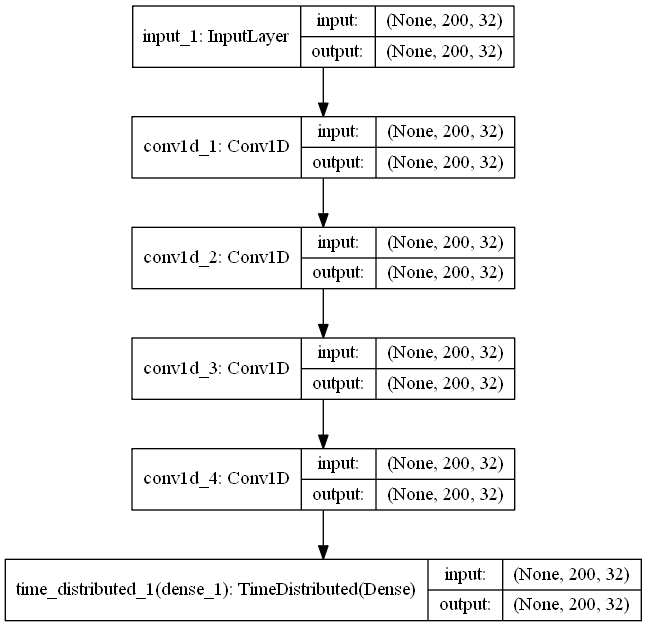
\includegraphics[width=0.8\columnwidth]{images/model.png}
    \caption{4 layer dilated convnet with \(seqLength=200\) and \(numFeatures=32\).}
    \label{fig.model}
    \end{figure}
  
  \section{Data}
  \label{sec:data}

  Our data are signals of vectors with \(numFeatures\) features. Each dataset is comprised of a normal signal and a "corrupted" signal of equal length. The datasets are obtained from two different sources.
  
  \subsection{Rook Data}
  \label{subsec:rookdata}

  The first source is data obtained from the authors of \cite{vines2015rook}. This data is a collection of recordings of client-side game network traffic from different play sessions, half of which are normal, and the other half are using the Rook system to insert messages into the traffic. These are UDP packets with payloads that use a custom network protocol unique to the game Team Fortess 2 \cite{TF2}. We do not know anything about this protocol, except that the payloads vary in length, which makes our feature vectors variable length.

  The normal signal in this case is the nomal game traffic, and the corrupted signal is the traffic containing hidden Rook messages.

  \subsection{Generated Data}
  \label{subsec:generateddata}

  Early experiments with the Rook dataset did not give good results with either of our methods, and indicated that this was primarily due to the dataset not being large enough relative to feature length and frequency of corrupted values. Therefore, we created a simple parametric signal generator to serve as a general representation of this problem on a smaller scale. Advantages of this approach are that we can generate as much data as desired, and that we can observe changes in results as we modulate parameters.

  We generate the normal signal by creating \(numFeatures\) 1D signals. Each signal has a randomly chosen period, waveform (sin, square, or sawtooth), midpoint, and amplitude. The signals are then concatenated along the feature axis. Alteratively, we can take the mean of the feature signals to make a 1D audio-like signal containing all of the features. We then create the corrupted signal by taking half of the normal signal, and randomly permuting 1 of the feature values at some regular interval. The permutation value could be random, or it could be set to some periodic signal to mimic the insertion of messages with some learnabe pattern.

  \section{Methods}
  \label{sec:methods}

  Our problem can be generalized to: We are given access to some limited amount of a multi-feature non-random signal that is known to be unaltered, and a limited amount of a new signal with similar shape and feature patterns (network traffic from the same application for example) that may or may not have had its data altered in some way. Without explicitly knowing anything about the meaning of the data, can we determine whether data has been altered in the new signal? We have developed 2 methods to solve this.

  \subsection{Method 1}
  \label{subsec:method1}

  The first method is the intuitive approach. We train a neural network on half of the known normal signal until it can fairly accurately predict the next sample in the sequence and thus has a decent understanding of the patterns in the features. We use a causal dilated convolutional network because this type of network has been shown to be effective for sequence prediction in a signal.
  
  Then, the remaining half of the known normal signal is split into two equal length subsets at a random position. We also take a section of this length from the unknown, potentially corrupted signal starting at a random position. We then run the network on these three selections and record the errors of the sample predictions. Specifically, we take the l2 norm of the difference between the second half (to ensure the convolution kernel is not driven by padded zeros) of the network output sequence and its corresponding position in the target signal, which is just the input signal shifted by 1. We then examine the difference between the prediction errors in the first and second normal signal selections, and the difference between the prediction errors in the first normal and the unknown signal selections.  We repeat this process with new random selections and continue collecting error comparisons in each category to avoid skewing our results toward a behavior in a particular section of the signal. If the absolute value of the mean of the normal vs. unknown comparison is significantly higher than the absolute value of mean of the normal vs. normal comparison, then the unknown signal likely has altered data. If there is little difference between the absolute values of the comparisons, then the unknown signal is likely not altered.

  In other words, let $A = \{\vec{a_0},...,\vec{a_{|A|}}\}$ be the set of known normal data and $B = \{\vec{b_0},...,\vec{b_{|B|}}\}$ be the set of new data in which we are trying to determine if there has been any alteration. The vectors $\vec{a} = (a_0,...,a_{numFeatures}),\vec{a}\in A$ and $\vec{b} = (b_0,...,b_{numFeatures}),\vec{b}\in B$ are feature vectors of length $numFeatures$.

  Define the following sets:
  
  $A_{train}=\{\vec{a_0},...,\vec{a_{\frac{|A|}{2}}}\},A_{train}\subset{A}$.

  Build our CNN (parameters defined in Section~\ref{sec:network}) with the loss function for given input data $X = \{\vec{x_0},...,\vec{x_{|X|}}\}$ defined as the mean squared error between the output and the target set $Y = \{\vec{x_1},...,\vec{x_{|X|}},\vec{x_0}\}$. The predictions are done in batches of width $seqLength$. Train this CNN with $A_{train}$ as the input data until it achieves relatively small error, and save the model.

  $A_{test1} = \{\vec{a_r},...,\vec{a_{r+\frac{|A|}{4}}}\},A_{test1}\subset{A}$, where $r$ is a random integer such that \(\frac{|A|}{2}<r<\frac{3|A|}{4}\).
  
  $A_{test2} = A \setminus (A_{train} \cup A_{test1}),A_{test2}\subset{A}$.

  $B_{test} = \{\vec{b_s},...,\vec{b_{s+\frac{|B|}{4}}}\},B_{test}\subset{B}$, where $s$ is a random integer such that $0<s<\frac{3|B|}{4}$,

  We now have our trained model perform predictions with $A_{test1}$ as the input data and record the list of mean squared errors between the 2\textsuperscript{nd} half of each batch of the predictions and the 2\textsuperscript{nd} half of each batch of the target data. This error list will be of length $n = \left \lfloor \frac{|A_{test1}|}{seqLength} \right \rfloor$. We also record the prediction errors for $A_{test2}$ and $B_{test}$
  
  For total of $m$ iterations, we then repeat the definition of $A_{test1}$, $A_{test2}$, and $B_{test}$ with new random indices $r$ and $s$, and repeat the prediction step, recording new respective error lists, giving a total of $m$ error lists for each input set. We record these error lists into the new size $m \times n$ matrices $C$, $D$, and $E$, respectively:

  $C \in \mathbb{R}^{m \times \left \lfloor \frac{|A_{test1}|}{seqLength} \right \rfloor}$, $c_{i,j} \in C$ is the mean squared error of the trained CNN's prediction of the 2\textsuperscript{nd} half of the $j^{th}$ batch of $A_{test1}$ at iteration $i$.

  $D \in \mathbb{R}^{m \times \left \lfloor \frac{|A_{test2}|}{seqLength} \right \rfloor}$, $d_{i,j} \in D$ is the mean squared error of the trained CNN's prediction of the 2\textsuperscript{nd} half of the $j^{th}$ batch of $A_{test2}$ at iteration $i$.

  $E \in \mathbb{R}^{m \times \left \lfloor \frac{|B_{test}|}{seqLength} \right \rfloor}$, $e_{i,j} \in E$ is the mean squared error of the trained CNN's prediction of the 2\textsuperscript{nd} half of the $j^{th}$ batch of $B_{test}$ at iteration $i$.

  Finally, we examine and compare attributes (such as mean, standard deviation, and RMS) of the error lists along the batch axis in our 3 new matrices across the 32 iterations, to get an idea of the general behavior.

  The main task is to look at:

  $knownComp_{i} = \frac{1}{n}\left(\sum\limits_{j=0}^n{c_{i,j}}\right) - \frac{1}{n}\left(\sum\limits_{j=0}^n{d_{i,j}}\right)$

  $knownAvg_{i} = \frac{\frac{1}{n}\left(\sum\limits_{j=0}^n{c_{i,j}}\right) + \frac{1}{n}\left(\sum\limits_{j=0}^n{d_{i,j}}\right)}{2}$

  $unknownComp_{i} = \frac{1}{n}\left(\sum\limits_{j=0}^n{e_{i,j}}\right) - \frac{1}{n}\left(\sum\limits_{j=0}^n{d_{i,j}}\right)$

  $unknownAvg_{i} = \frac{\frac{1}{n}\left(\sum\limits_{j=0}^n{e_{i,j}}\right) + \frac{1}{n}\left(\sum\limits_{j=0}^n{d_{i,j}}\right)}{2}$

  $corruptionFactor = \frac{1}{m}\sum\limits_{i=0}^m{\left(\frac{unknownComp_{i}}{unknownAvg_{i}} - \frac{knownComp_{i}}{knownAvg_{i}}\right)}$
  
  The value of $corruptionFactor$ is essentially the measure of how poorly our trained network is able to predict our unknown data relative to our known data, and indicates whether the set of unknown data contains values that have been altered by some means. In general, the higher the value, the more likely it is that data has been altered. However, this relationship is highly dependent on multiple factors. Primarily, as the values of $|A|$, $|B|$, $\frac{1}{numFeatures}$, and $corrFreq$ (the percentage of data that has been altered in the event of altered data) decrease, so will the gap between the $corruptionFactor$ in the unaltered case and the $corruptionFactor$ in the altered case. But, given sufficiently high values in these variables and an empirically derived threshold, this method is reliable to confidently classify the presence of altered data.

  As an alternative to taking the mean along the iteration axis, it is useful to look at the graph of scaled mean comparisons, $\frac{unknownComp_{i}}{unknownAvg_{i}}$ and $\frac{knownComp_{i}}{knownAvg_{i}}$ across the iterations. Results are discussed in Section~\ref{subsec:method1results}.

  \subsection{Method 2}
  \label{subsec:method2}

  The second method requires less data than the first to achieve a solution with similar reliability. The unknown data and known data are each divided into two equal parts at a random index. We use the same CNN architecture as before, but this time we use 3 networks:
  \begin{itemize}
   \item $modelKU$ is trained on the union of the 1st half of the known and 1st half of the unknown data.
   \item $modelKK$ is trained on all of the known data.
   \item $modelUU$ is trained on all of the unknown data.
  \end{itemize}
  We then collect prediction errors using the 2nd half of each batch as in the first method. Again, the training and prediction is done over $m$ iterations resulting in $m$  error lists of length $n$ of each type. The divided data is shuffled at each iteration, but the initial bisections of the known and unknown datasets are retained.
  
  Let each of the following variables refer to the $i^{th},j^{th}$ element in the $m \times n$ matrix of mean squared prediction errors of the given model and data type.
  \begin{itemize}
    \item ${knownA_{KU}}_{i,j}$ : $modelKU$ on 1st half of \textbf{known} data.
    \item ${unknownA_{KU}}_{i,j}$ : $modelKU$ on 1st half of \textbf{unknown} data.
    \item ${knownA_{KK}}_{i,j}$: $modelKK$ on 1st half of \textbf{known} data.
    \item ${knownB_{KK}}_{i,j}$: $modelKK$ on 2nd half of \textbf{known} data.
    \item ${unknownA_{UU}}_{i,j}$: $modelUU$ on 1st half of \textbf{unknown} data.
    \item ${unknownB_{UU}}_{i,j}$: $modelUU$ on 2nd half of \textbf{unknown} data. 
  \end{itemize}
  
  We can learn much about our data by extracting different attributes of these errors. Of primary interest is the comparison of the differences between means of certain pairs of error lists scaled by the overall average means of the union of the pairs. In other words:

  At some iteration $i$,

  $ukComp_i = \frac{\frac{1}{n}\left(\sum\limits_{j=0}^n{{unknownA_{KU}}_{i,j}}\right) - \frac{1}{n}\left(\sum\limits_{j=0}^n{{knownA_{KU}}_{i,j}}\right)}{\frac{1}{2n}\left(\sum\limits_{j=0}^n{{unknownA_{KU}}_{i,j}}\right) + \frac{1}{2n}\left(\sum\limits_{j=0}^n{{knownA_{KU}}_{i,j}}\right)}$

  $kkComp_i = \frac{\frac{1}{n}\left(\sum\limits_{j=0}^n{{knownB_{KK}}_{i,j}}\right) - \frac{1}{n}\left(\sum\limits_{j=0}^n{{knownA_{KK}}_{i,j}}\right)}{\frac{1}{2n}\left(\sum\limits_{j=0}^n{{knownB_{KK}}_{i,j}}\right) + \frac{1}{2n}\left(\sum\limits_{j=0}^n{{knownA_{KK}}_{i,j}}\right)}$

  $uuComp_i = \frac{\frac{1}{n}\left(\sum\limits_{j=0}^n{{unknownB_{UU}}_{i,j}}\right) - \frac{1}{n}\left(\sum\limits_{j=0}^n{{unknownA_{UU}}_{i,j}}\right)}{\frac{1}{2n}\left(\sum\limits_{j=0}^n{{unknownB_{UU}}_{i,j}}\right) + \frac{1}{2n}\left(\sum\limits_{j=0}^n{{unknownA_{UU}}_{i,j}}\right)}$

  While it may seem strange to observe predictions on the same data that was used to train the network, this is the trick to the method. We are not actually interested in creating a reliable predictive network as in the first method, rather we are interested in observing how the predictive behavior of different networks develop relative to pairs of input data, and what that can tell us about the data.
  
  If a network is trained on two different sets of data that are shuffled together, and then we examine the network's prediction accuracy on the same two datasets separately (and we repeat this for several iterations reshuffling and retraining every time), three different behaviors emerge:
  
  \begin{enumerate}
    \item The difference in errors stays around 0, and there is some variance. This happens in the case where both datasets have similar behavioral features (such as two samples of a signal from the same source), and those features are clear and learnable. The network will tend to 'prefer' one of the samples at each iteration, but when observed over many iterations will average out to 0. This is the behavior we expect from $kkComp$.
    \item The difference in errors stays around 0, and there is very little variance. This happens in the case where both datasets have similar behavioral features, but the features are not as easily learnable (such as in the case of random data permutation). Because the features are more difficult to learn, the network is less likely to 'prefer' one of the datsets over the other at a given iteration, but it will still average out to zero across the iterations. This is the behavior we would expect from $uuComp$ in the cases where the unknown data has been altered.
    \item The difference in errors centers on a value much higher or lower than zero, and there is some variance. This happens in the case where both datasets have similar overall features, but one is consistently more easily learnable than the other (such as in the case where only one sample has permuted values). On average across the iterations, the network will 'prefer' the more consistent dataset, and will have higher prediction errors on the other. If we are looking at datasetA - datasetB, a higher average indicates corruption in datasetA, and a lower average indicates corruption in datasetB. This is the behavior we would expect from $ukComp$ in the cases where the unknown data has been altered.
  \end{enumerate}

  In general, if the $ukComp$ value is consistently higher than the other two comparisons across the iterations, it indicates the presence of altered data in the unknown sample. If there was no altered data, all three values would be centered around 0. We can examine the means or the plots of the $ukComp$, $kkComp$, and $uuComp$ values across the iterations. Results are discussed in Section~\ref{subsec:method2results}.

  \section{Results}
  \label{sec:results}

  Both methods were able to reliably detect the presence of altered data given sufficient dataset size and frequency of permutation.

  \subsection{Method 1 Results}
  \label{subsec:method1results}

  Figure~\ref{fig.scaledmeancomp-NN} shows such graphs of scaled mean comparisons, $\frac{unknownComp_{i}}{unknownAvg_{i}}$ and $\frac{knownComp_{i}}{knownAvg_{i}}$ across the iterations for the two cases where the unknown data has and hasn't been altered. We see little separation between the known and unknown comparisons in the non-altered case (Top), and clear separation in the altered case (Bottom), which aligns with our expectation.

  \begin{figure}[h]
    \centering
    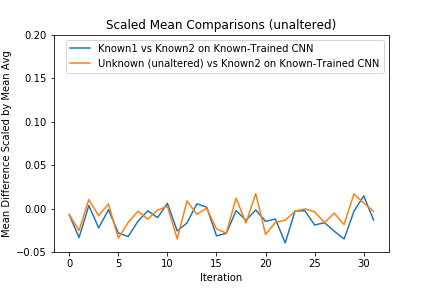
\includegraphics[width=0.8\columnwidth]{images/SMC-rvnNN-nvnNN-unalt.png}
    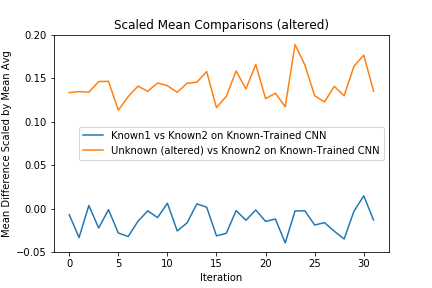
\includegraphics[width=0.8\columnwidth]{images/SMC-rvnNN-nvnNN-alt.png}
    \caption{Known vs known and unknown vs known mean comparisons scaled by relative avg means, across 32 iterations, in the cases where (Top) the unknown data has not been altered and (Bottom) the unknown data contains altered values. The unknown vs known comparison in the bottom image is significantly higher, indicating the presence of altered data.}
    \label{fig.scaledmeancomp-NN}
    \end{figure}
  
  \subsection{Method 2 Results}
  \label{subsec:method2results}
  
  Figure~\ref{fig.diff3Comp} shows the plot of the 3 comparisons, $ukComp$, $kkComp$, and $uuComp$, in the two cases where the unknown data has and hasn't been altered. We observe that in the non-altered case (Top), the 3 values have little difference and all stay around 0, while in the altered case (Bottom), the $ukComp$ value is consistently higher than the other two comparisons, aligning with our expectation.

  \begin{figure}[h]
    \centering
    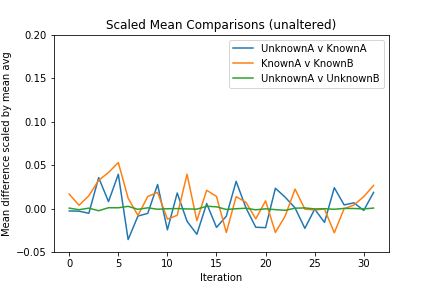
\includegraphics[width=0.8\columnwidth]{images/diff3CompUnaltered.png}
    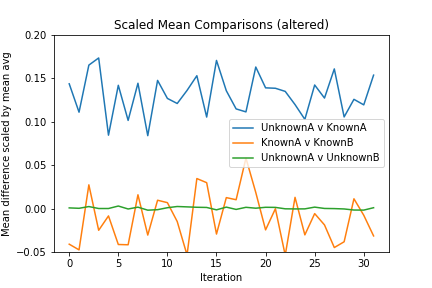
\includegraphics[width=0.8\columnwidth]{images/diff3Comp.png}
    \caption{Mean comparisons scaled by relative avg means, across 32 iterations, in the cases where (Top) the unknown data has not been altered and (Bottom) the unknown data contains altered values. Each pair of data subsets is predicted by a network trained on that pair. In the altered case, the unknown v known pair has a significant and consistent higher difference than the pairs operating on only known or only unknown data. This correctly indicates that the unknown set contains altered data.}
    \label{fig.diff3Comp}
    \end{figure}

  \section{Conclusion and Future work}
  \label{sec:conclusion}
  
  We have described 2 methods which can reliably detect the presence of data alteration in a signal.
  
  \bibliography{refs}
  \bibliographystyle{plain}
  
  \end{document}